\documentclass{homework}
% \usepackage{graphicx} % Required for inserting images
\usepackage{amsmath}
\usepackage{gensymb}
\usepackage{subfig}
\usepackage{float}
\usepackage{pythonhighlight}

\class{APPM 5630}
\title{Homework 1-2}
\author{Sean Jennings}
\date{January 28, 2025}

\begin{document}
\maketitle

(NOTE: I didn't realize that homeworks 1 and 2 were intended to be submitted separately. I've included them together
and submitted the same document for each assignment on GradeScope. Hopefully this doesn't cause any issue!)

\section{Problem 1}
Let $C$ be a set and $L$ be any line. First, we show the forward direction:
that if $C$ is convex, $C \cap L$ also is. Well, since a line is a convex
set, this follows immediately from the fact that intersection preserves
convexity.

In the reverse direction, assume that $C \cap L$ is convex for every line $L$. We want
to show that $C$ is convex. Let $x,y\in C$. Choose $L$ to be the unique line that
passes through both $x$ and $y$. Now, since $x, y \in C \cap L$, for each $\lambda \in [0,1]$,
we have $\lambda x + (1 - \lambda) y \in C \cap L$ by the convexity of $C \cap L$. 
Therefore, $\lambda x + (1 - \lambda) \in C$  and $C$ is convex.

\section{Problem 2}
\begin{letterenum}
\item Graphically, it is easy to see that $\{y_1 a_1 + y_2 a_2 | -1 \leq y_1 \leq 1, -1 \leq y_2 \leq 1\}$
is a polyhedra (figure \ref{figure:poly}). It is contained in the half-plane spanned by $a_1$ and $a_2$ and constrained
by half spaces where $y_1$ and $y_2$ are between -1 and 1.


\begin{center}
    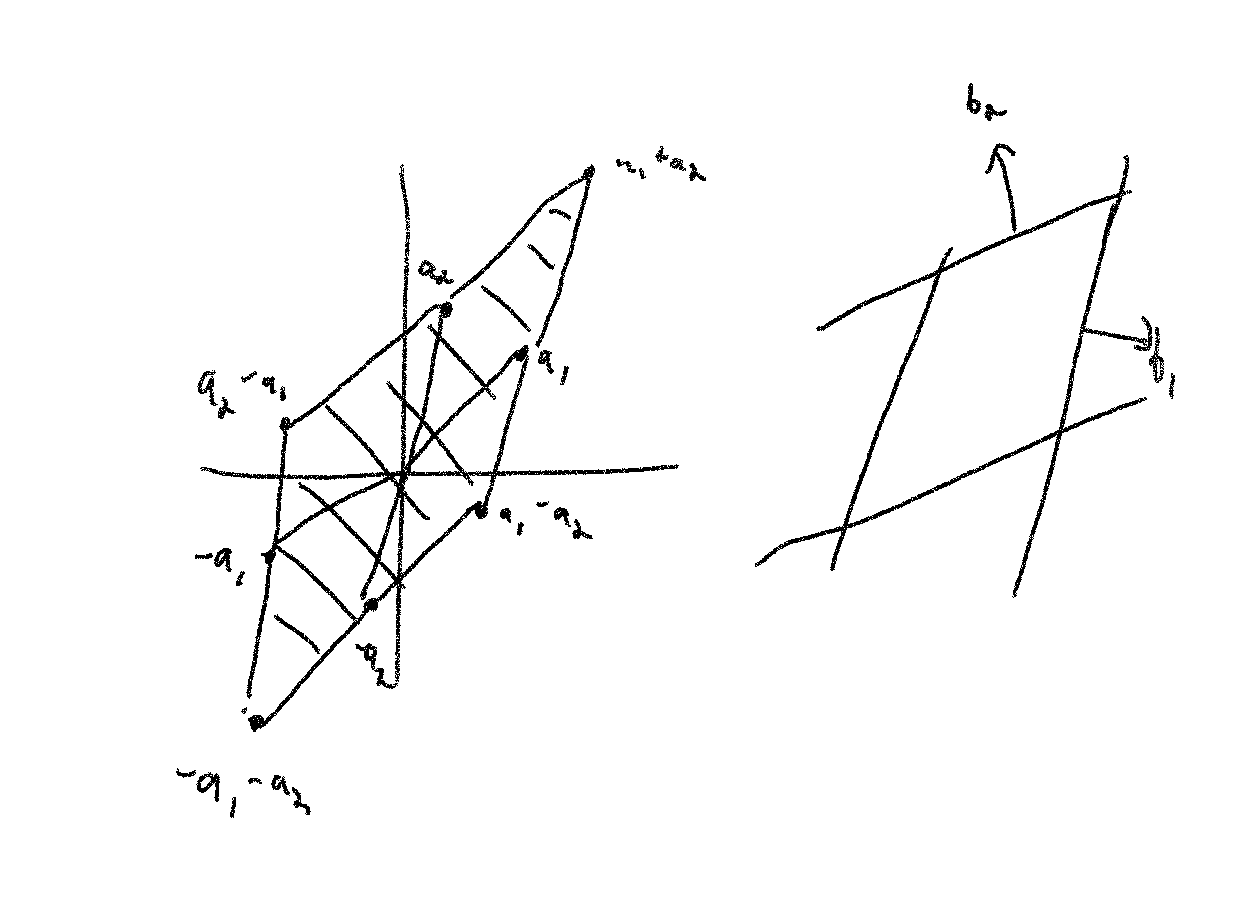
\includegraphics[width=0.6\linewidth]{images/polyhedra.png}
    \captionof{figure}{Constrained linear combination problem 2a.}
    \label{figure:poly}
\end{center}

In terms of the standard form $A x \preceq b$, $Fx = g$, to compute the matrix $A$, we must find
the normal vectors of the constraining halfspaces. We denote the component of $a_1$ which is
orthogonal to $a_2$ as $\text{oproj}_{a_2} a_1$ and vice-versa. This can be computed as
\begin{equation*}
    \text{oproj}_{a_2} a_1 = a_1 - \text{proj}_{a_2} a_1 = a_1 - \frac{a_1 \cdot a_2}{||a_2||^2} a_2
\end{equation*}
Let $b_1 = \text{oproj}_{a_2} a_1$ and $b_2 = \text{oproj}_{a_1} a_2$.
Normalize $b_1$ and $b_2$ to obtain $\hat{b}_1$ and $\hat{b}_2$ (e.g. $\hat{b}_1 = b_1 / ||b_1||_2$)
Then, the inequality constraint $A x \preceq b$ is given by:
\begin{equation*}
    \mat{\hat{b}_1 \\ \hat{b}_2 \\ - \hat{b}_1 \\ - \hat{b}_2} x \preceq
        \mat{||b_1||_2 \\ ||b_2||_2 \\ ||b_1||_2 \\ ||b_2||_2}
\end{equation*}

Let the rows of $F$ be a basis for the subspace orthogonal to span$(\{a_1, a_2\})$. Then, the hyperplane
constraint is given by $Fx = 0$.

\item The given set is a polyhedron since it is the intersection of halfspaces and hyperplanes. To see this,
let $a = [a_1 \dots a_n]^T$. Each equation
\begin{align*}
    \mathbf{1}^T x &= 1 \\
    a^T x &= b_1 \\
    [a_1^2 \dots a_n^2] x &= b_2
\end{align*}
defines a hyperplane and $x \succeq 0$ defines the positive orthant which is the intersection
of half-spaces.

In the standard form, take $A$ to be the negative identity matrix, $b$ to be 0. $F$ and $g$
can be found by vectorizing the above equalities, i.e.
\begin{equation*}
    F = \mat{
        \mathbf{1}^T \\
        a^T \\
        a_1^2 & \dots & a_2^2
    }, \qquad g = \mat{1 \\ b_1 \\ b_2}
\end{equation*}

Note: it's possible that this polyhedron is empty if $F$ is not full rank, or if the
intersection of these hyperplanes do not intersect the positive orthant. 

\item By the Cauchy-Schwarz inquality, we have:
\begin{equation*}
    x^T y \leq |x^T y| \leq ||x||_2 ||y||_2 = ||x||_2
\end{equation*}

But $x^T y$ also takes its maximum when $y$ is in the same direction as $x$, i.e. when $y = x / ||x||_2$.
In this case, $x^T y = x^T x / ||x||_2 = ||x||_2$. Therefore, $x^T y \leq 1$ for all $y$ iff $||x||_2 \leq 1$.
Thus, the given set is the intersection of the
unit ball ($\{x | ||x||_2 \leq 1\}$) with the positive orthant, which is clearly not a polyhedra.

\item By the triangle inequality, we have the following for all $y$ with $||y||_1 = 1$:
\begin{align*}
    x^T y \leq |x^T y | = \biggl| \sum_{i=1}^n x_i y_i \biggr| &\leq \sum_{i=1}^{n} |x_i | |y_i| \\
        &\leq |x_j| \sum_{i=1}^{n} y_i = ||x||_{\infty}
\end{align*}
where $j = \text{argmax}_i x_i$ is the index of the largest component of $x$. This relation is
attained as an equality when $y=e_j$ (where $e_j$ is the $j$th standard unit vector).
Then, analogous to the part c), we have $x^T y \leq $ for all $y$ if and only if $||x||_{\infty} \leq 1$,
or equivalently if and only if $x_i \leq 1$ for each $i=1,\dots,n$.

Therefore, this set is indeed a polyhedron. Take
\begin{equation*}
    A = \mat{
        I & 0 \\
        0 & -I
    }, \qquad b = \mat{\mathbf{1} \\ 0}.
\end{equation*}
where $I$ is the $n$ by $n$ identity matrix.


\end{letterenum}

\section{Problem 3}
\begin{letterenum}
\item For the first three parts, we will use the fact that the intersection of convex sets is also convex.
The slab, rectangle, and wedge can all be viewed as the intersection of halfspaces and are therefore convex.
\item $\dots$
\item $\dots$
\item Let $C$ be the given set $\{x | ||x - x_0||_2 \leq ||x - y||_2 \quad \forall y \in S\}$. Let $x_1$ and
$x_2$ be points in $C$, and $z = \lambda x_1 + (1 - \lambda) x_2$ ($\lambda \in [0, 1]$) be a convex
combination. Then, applying the triangle inequality,
\begin{align*}
    ||z - x_0|| &= ||\lambda x_1 + (1 - \lambda) x_2 - x_0|| \\
        &\leq \lambda ||x_1 - x_0|| + (1 - \lambda) ||x_2 - x_0|| \\
        &\leq [\lambda + (1 - \lambda)] \max_{i\in \{1,2\}} ||x_i - x_0|| \\
        &= \max_{i\in \{1,2\}} ||x_i - x_0|| \\
        &\leq || y - x_0||
\end{align*}

Thus, $z \in C$ and $C$ is convex.

In simple terms, any point on the line segment connected $x_1$ and $x_2$ must be at least
as close to $x_0$ as the further of the two endpoints, and is therefore closer to $x_0$
than to $S$.

\item If $S$ is not convex, then it can easily happen that the set of points closer to $S$ than
to $T$ is also nonconvex. Take for instance $S = \{x | |x| \geq 2\} \subset \R$ and $T = \{ 0 \}$.
Then, the set of points closer to $S$ is $\{x | |x| \geq 1\}$ which is clearly not convex.

\item Let $C = \{x | x + S_2 \subseteq S_1\}$ where $S_1$ is convex. Let $x,y \in C$
and $z=\lambda x + (1 - \lambda) y$ for some  $\lambda \in [0,1]$. Then, for all $x\in S_2$,
we have $x+s \in S_1$ and $y + s \in S_1$. By rthe convexity of $S_1$, we have
$\lambda (x + s) + (1 - \lambda) (y+s) \in S_1$. But
\begin{align*}
    \lambda (x + s) + (1 - \lambda) (y+s) &= \lambda x + (1 - \lambda) y + [\lambda + (1 - \lambda)] s \\
        &= z + s
\end{align*}
So $z+s\in S_1$ for all $s \in S_2$, which implies $z+S_2\subseteq S_1$, $z \in C$, thus $C$ is convex.

\item This set is also convex by very similar logic to part d). Each $z$ which is a convex combination
of some $x_1$ and $x_2$ in the given set is at least as close to $a$ as the further of $x_1$ and $x_2$.
Since the distance of $x_1$ and $x_2$ to $a$ does not exceed a fixed fraction of their distance
to $b$, the same must hold for $z$.

\end{letterenum}

\section{Problem 4}
The convex hull of rank-$k$ outer products is the set of all positive semidefinite matrices
with rank greater than or equal to $k$.

To see that $X X^T$ is PSD, write $X$ in terms of its SVD, $X = U\Sigma V^T$, where $U\in\R^{n \times n}$
and $V \in \R^{k \times k}$ are orthogonal matrices and $\Sigma \in \R^{n\times n}$ has entries
\begin{equation*}
    \Sigma_{ij} = \biggl\{
        \begin{array}{ll}
            \sigma_i &\qquad \text{if } i = j \leq k \\
            0 &\qquad \text{otherwise}
        \end{array}
    \biggr.
\end{equation*}

Therefore,
\begin{align*}
    XX^T &= U\Sigma V^T V \Sigma^T U^T \\
        &= U \Sigma^2 U^T
\end{align*}
Thus, the eigenvalues of the outer product $XX^T$ are the square of the singular values of $X$, and are thus
all positive, which shows $XX^T$ is PSD.

The conic hull of outer products is the set of all matrices of the form
$\sum_{i=1}^m \theta_i X_i X_i^T$ with $\theta_i \geq 0$. To show this matrix is PSD, note 
that for any $z \in \R^n$, we have
\begin{equation*}
    z^T \biggl( \sum_{i=1}^{m} \theta_i X_i X_i^T \biggr) z =
        \sum_{i=1}^{m} \theta_i \biggl(z^T X_i X_i^T z\biggr) \geq 0
\end{equation*}

since each $z^T X_i X_i^T z \geq 0$.

To see that the rank of the conic combination may be larger than $k$, we will give an example
with $n = 2$ and $k=1$:
\begin{equation*}
    \mat{1 \\ 0} \mat{1 & 0 } + \mat{0 \\ 1} \mat{0 & 1} = \mat{1 & 0 \\ 0 & 0} + \mat{0 & 0 \\ 0 & 1} = \mat{1 & 0 \\ 0 & 1}
\end{equation*}


\section{Homework 2 -- Problem 1}
Figure \ref{fig:python} shows Python code which solves the optimization problems
$\min_{\beta_p} ||y - X \beta_p||_p$ for $p\in\{1,2\}$, with $p=1$ and $p=2$ corresponding to
$\ell_1$ and $\ell_2$ norms, respectively.

The code reads the downloaded csv file with $m=4898$ rows corresponding to different wine varieties. 
It extracts the first $n=11$ columns as the feature
matrix $X\in \R^{m \times n}$, with each column corresponding to a physicochemical property of the wine, and $y\in\R^m$
as the final column in the CSV file, indicating the quality of the wine. Finally, the optimization problem
is solved for each norm.

\begin{center}

\begin{python}
import pandas as pd
from pathlib import Path
import matplotlib.pyplot as plt
import cvxpy as cp

df = pd.read_csv(DATA_DIR / "winequality-white.csv", sep=';')
# df = df[np.logical_and(df['quality'] > 3, df['quality'] < 9)]

n = 11
X = df.iloc[:, :n].to_numpy()
betas = [
    cp.Variable(n),
    cp.Variable(n)
]
y = df.iloc[:, n].to_numpy()

objectives = [cp.Minimize(cp.norm(y - X @ betas[i], p=p))
             for i, p in enumerate([1,2])]
problems = [cp.Problem(obj) for obj in objectives]
results = [prob.solve() for prob in problems]
\end{python}

\captionof{figure}{Python code}
\label{fig:python}
\end{center}

Figure \ref{figure:hist} shows a histogram of the residuals $y - X \beta_p$ for $p\in\{1,2\}$.
Visually, the results norm do not seem very different. The residuals are spread rather evenly
between values less than 1, where the $\ell_1$ norm dominates $\ell_2$, and values greater than 1, where $\ell_2$
dominates. This observation may explain why the solution $\beta_1$ which optimizes the 1-norm and $\beta_2$ which
optimizing the 2-norm are close together. The proximity of the solutions is corroborated by the results in figure {}.


\begin{center}
    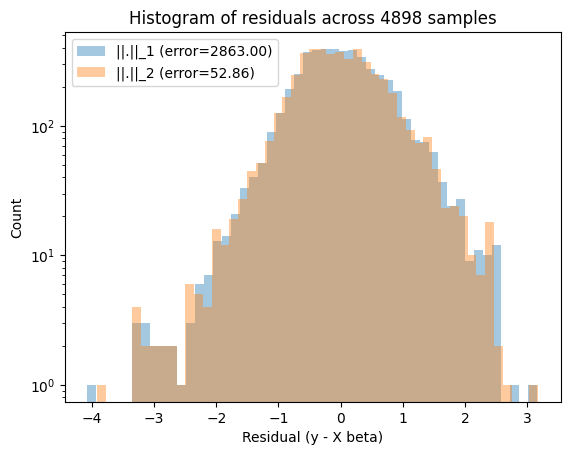
\includegraphics[width=0.5\linewidth]{images/histogram.png}
    \captionof{figure}{Histogram of residuals}
    \label{figure:hist}
\end{center}

\begin{center}
    \begin{python}
for p in [1,2]:
    for i in [0,1]:
        norm_eval = np.linalg.norm(y - X @ betas[i].value, ord=p)
        print(f"||y - X beta_{i+1}||_{p} = {norm_eval}")

>>> ||y - X beta_1||_1 = 2863.0000933377737
>>> ||y - X beta_2||_1 = 2872.505472032642
>>> ||y - X beta_1||_2 = 53.01847030586845
>>> ||y - X beta_2||_2 = 52.861550406976

    \end{python}
    \label{figure:python-output}
    \captionof{figure}{Comparison of norm evaluations ($p\in\{1,2\}$) across solutions $\beta_1, \beta_2$}
\end{center}


As seen in figure \ref{fig:wine-quality-dist}, the distribution of wine qualities is heavily favored
towards values in the middle of the scale, with less than 1\% rated at 3 and 9.
The residual histogram is plotting again in figure \ref{figure:hist-filt}
with these infrequently occurring wine qualities of 3 and 9 removed
(see commented line in figure \ref{fig:python}).

The infrequently occurring wine qualities 
seem to correspond to the residual components with the greatest magnitude,
as the more extreme residual values of -4 and positive 3 appear in figure \ref{figure:hist}, but not
figure \ref{figure:hist-filt}. However, the overall proximity of the residual distributions remains
largely unchanged.

\begin{center}
    \begin{python}
counts, _ = np.histogram(y, bins=[2.5 + i for i in range(8)]) 
count_df = pd.DataFrame({'count': counts, 'fraction': counts / len(y)}, index=np.arange(3, 10))
count_df.index.name = "quality"
print(count_df)

>>> quality   count  fraction
>>> 3           20   0.0041
>>> 4          163   0.0333
>>> 5         1457   0.2975
>>> 6         2198   0.4488
>>> 7          880   0.1797
>>> 8          175   0.0357
>>> 9            5   0.0010
    \end{python}
    \captionof{figure}{Distribution of wine qualities}
    \label{fig:wine-quality-dist}
\end{center}

\begin{center}
    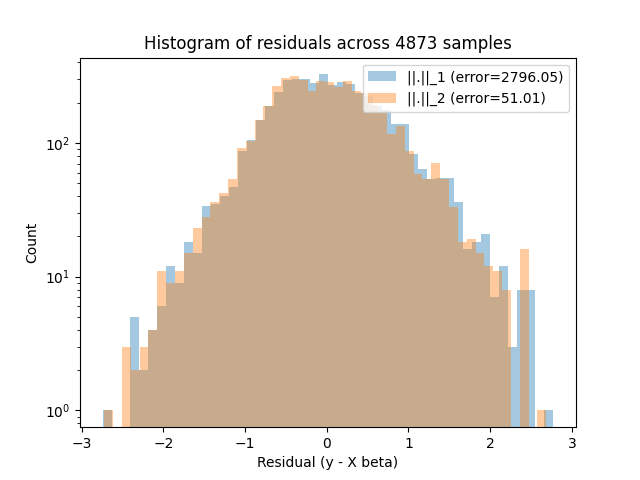
\includegraphics[width=0.6\linewidth]{images/histogram_filtered.png}
    \captionof{figure}{Histogram of residuals with wine qualities of 3 and 9 removed}
    \label{figure:hist-filt}
\end{center}











\end{document}
